\appendix

	% Add your appendices here. You must leave the appendices enclosed in the appendices environment in order for the table of contents to be correct.
	
\begin{appendices}
%\chapter{Appendices I} \label{app:appendix_one}
%\section{A1} \label{ase:app_one_sect_1}

\chapter{Multiple changepoints} \label{app:mQCP}

In this appendix, we propose heuristics for the case of multiple changepoints and demonstrate their performance.
We consider the following states
\begin{align}
    \label{eq:ch3_QSD-theta_states}
    \ket{\psi} = \ket{0}, \quad \ket{\phi_k} = \cos(k \theta) \ket{0} + \sin(k \theta) \ket{1},\ k \in \{1, \dots, p\}.
\end{align} 

Consider the case where Alice promises Bob $N$ copies of the state $\ket{0}$.
Bob suspects the following:
(1) At some point $c_1$, her device might have mutated from generating the state $\ket{0}$ to the state $\ket{+}$.
(2) At a different point $c_2$, a further mutation might have caused the switch from the state $\ket{+}$ to the state $\ket{1}$.
(3) At a third point $c_3$, one last mutation could have led to $\ket{1}$ turning it to $-\ket{-}$.
The possible mutations are as described in Figure~\ref{fig:ch3_QSD-pi_4_states}.

\def\xmax{2.0}
\def\ul{0.6}
\def\R{2.0}
\def\ang{45}

\begin{figure}[h]
    \centering
    \begin{tikzpicture}
        % coordinates
        \coordinate (O) at (0,0);
        \coordinate (zero) at (\xmax,0);
        \coordinate (plus) at (\ang:\R);
        \coordinate (one) at (0,\xmax);
        \coordinate (neg_minus) at (3*\ang:\R);
  
        % axis
        \draw[->] (-1.5*\xmax,0) -- (1.5*\xmax,0);
        \draw[->] (0,-1.5*\xmax) -- (0,1.5*\xmax);
  
        % zero state
        \node[above right] at (zero) {$\ket{0}$};
        \draw[vector] (O) -- (zero);
        % plus state
        \node[above right] at (plus) {$\ket{+}$};
        \draw[vector] (O) -- (plus);
        % one state
        \node[above right] at (one) {$\ket{1}$};
        \draw[vector] (O) -- (one);
        % negative minus state
        \node[above left] at (neg_minus) {$-\ket{-}$};
        \draw[vector] (O) -- (neg_minus);

        % angle
        \draw pic[->,"$\frac{\pi}{4}$",draw=black,angle radius=21,angle eccentricity=1.2] {angle=zero--O--plus};

        % circle
        \draw[dashed] (O) circle (\R);
    \end{tikzpicture}
    \caption{The state $\ket{0}$ promised by Alice and the possible mutated states $\ket{+}, \ket{1}$ and $-\ket{-}$ that Bob suspects of receiving.}
    \label{fig:ch3_QSD-pi_4_states}
\end{figure}

Upon receiving all of the $N$ states, Bob can exploit our framework by considering the following states
\begin{equation}
    \label{eq:ch3_QSD-Bob's_suspicion_succinct}
    \begin{aligned}
        \ket{\tau_{c_1 c_2 c_3}} = -\ket{0}^{\otimes c_1}\ \otimes \ket{+}^{\otimes (c_2 - c_1)}\ \otimes \ket{1}^{\otimes (c_3 - c_2)}\ \otimes \ket{-}^{\otimes (N - c_3)} %\\
        \quad (c_1, c_2, c_3) \in \Iset_N
    \end{aligned}
\end{equation}

When no changepoints occur, Bob is looking for the state
\begin{align}
    \label{eq:ch3_QSD-no_CP_eg}
    \ket{\tau_{N N N}} = \ket{0}^{\otimes N}.
\end{align}
If he suspects a mutation to the state $\ket{+}$, he looks for
\begin{align}
    \label{eq:ch3_QSD-1CP_eg}
    \ket{\tau_{c_1 N N}} = \ket{0}^{\otimes c_1}\ \otimes \ket{+}^{\otimes (N - c_1)}.
\end{align}
A suspicion of a further mutation to state $\ket{1}$ requires looking for the state
\begin{align}
    \label{eq:ch3_QSD-2CP_eg}
    \ket{\tau_{c_1 c_2 N}} = \ket{0}^{\otimes c_1}\ \otimes \ket{+}^{\otimes (c_2 - c_1)}\ \otimes \ket{1}^{\otimes (N - c_2)}.
\end{align}
When Bob suspects that all of the possible mutations may have occurred, he looks for
\begin{align}
    \label{eq:ch3_QSD-3CP_eg}
    \ket{\tau_{c_1 c_2 c_3}} = - \ket{0}^{\otimes c_1}\ \otimes \ket{+}^{\otimes (c_2 - c_1)}\ \otimes \ket{1}^{\otimes (c_3 - c_2)}\ \otimes \ket{-}^{\otimes (N - c_3)}.
\end{align}

\begin{comment}
\section{At most one changepoint}

Here, we look at the case when Bob suspects Alice's device of either having no mutations or ones that generate $\ket{+}$.
So Bob needs to determine exactly where this changepoint occurred.
This is accomplished by discriminating between the states described by Eq.~\eqref{eq:ch3_QSD-no_CP_eg} and Eq.~\eqref{eq:ch3_QSD-1CP_eg}.

We consider the closer-the-better reward strategy described in Eq.~\eqref{eq:ch3_QSD-R_ME_SD} to obtain
\begin{align}
    \label{eq:ch3_QSD-1CP_ctbr}
    R_{ij} =
    \begin{cases}
        \left( \frac{1}{\sqrt{2}} \right)^{|i-j|}, & i \in \{1, \dots, N\} \\
        0, & i = N+1
    \end{cases}
\end{align}
for $j \in \{1, \dots, N\}$.
\end{comment}

We discuss the case of identifying at most one changepoint in Section~\ref{sec:ch3_QSD-1CP}.

\section{At most two changepoints}\ref{sec:ch3_QSD-2CP}

When dealing with the scenario where at most two changepoints can occur, Bob must focus on the following states
\begin{equation}
    \label{eq:ch3_QSD-2CP}
    \begin{aligned}
        \ket{\tau_{c_1 c_2}} &\coloneqq \ket{\tau_{c_1 c_2 N \cdots N}} = \ket{\psi}^{\otimes c_1}\ \otimes \ket{\phi_1}^{\otimes (c_2 - c_1)}\ \otimes \ket{\phi_2}^{\otimes (N - c_2)}, \quad (c_1, c_2) \in \Iset_N.
    \end{aligned}
\end{equation}

Note here that
\begin{align}
    \ket{\tau_{c_1}} \coloneqq \ket{\tau_{c_1 N}} = \ket{\psi}^{\otimes c_1}\ \otimes \ket{\phi_1}^{\otimes (N - c_1)}
\end{align}
denotes the sequences corresponding to a single changepoint and
\begin{align}
    \ket{\tau_N} \coloneqq \ket{\tau_{N N}} = \ket{\psi}^{\otimes N} 
\end{align}
indicates the sequence with no changepoint.

\paragraph{Gram matrix.}

The Gram matrix can be computed using the formula,

\begin{align}
    \label{eq:ch3_QSD-T_ijkl}
    (T_{2CP})_{ij,kl} =
    \begin{cases}
        \gamma_1^{|i-j|}\ \gamma_2^{|j-k|}\ \gamma_{12}^{|k-l|}, &j < k \\
        \gamma_1^{|i-k|}\ \gamma_{12}^{|j-l|},\ \hspace{30pt} &\text{otherwise}
    \end{cases} 
\end{align}
where we have assumed for simplicity that the overlaps, $\gamma_1, \gamma_2$ and $\gamma_{12}$ are all non-negative real numbers. 
We proved that this assumption is without loss of generality in the one changepoint case (Lemma~\ref{lem:ch3_QSD-T_sym_Toep}), assuming it here makes the technical analysis a bit tidier. 

When represented as a matrix, we obtain a symmetric block matrix as illustrated in Eq.~(\ref{eq:ch3_QSD-T_2CP}).
\begin{align}
    \label{eq:ch3_QSD-T_2CP}
    T_{2CP} =
    \begin{pmatrix}
        T_{11} & T_{12} & T_{13} & \cdots & T_{1,N-2} & T_{1,N-1} & \rvline & T_{1N} \\
        T_{12}^\top & T_{11}^{(1)} & T_{12}^{(1)} & \cdots & T_{1,N-3}^{(1)} & T_{1,N-2}^{(1)} & \rvline & T_{2N} \\
        T_{13}^\top & T_{12}^{(1)\top} & T_{11}^{(2)} & \cdots & T_{1,N-4}^{(2)} & T_{1, N-3}^{(2)} & \rvline & T_{3N} \\
        \vdots & \vdots & \vdots & \ddots & \vdots & \vdots & \rvline & \vdots \\
        T_{1,N-2}^\top & T_{1,N-3}^{(1)\top} & T_{1,N-4}^{(2)\top} & \cdots & T_{11}^{(N-2)} & T_{12}^{(N-2)} & \rvline & T_{N-2,N} \\
        T_{1,N-1}^\top & T_{1,N-2}^{(1)\top} & T_{1,N-3}^{(2)\top} & \cdots & T_{12}^{(N-2)\top} & T_{11}^{(N-1)} & \rvline & T_{N-1,N} \\
        \hline
        T_{1N}^\top & T_{2N}^\top & T_{3N}^\top & \cdots & T_{N-2,N}^\top & T_{N-1,N}^\top & \rvline & 1 \\
    \end{pmatrix}. 
\end{align}
Each block, denoted by $T_{ik}$, is an $(N-i) \times (N-k)$ Toeplitz matrix.
The block $T_{11}$ is a symmetric Toeplitz matrix where each entry $(T_{11})_{jl} = \gamma_{12}^{|j-l|}$.
The notation $T_{ik}^{(n)}$ indicates the matrix obtained by discarding the \emph{last} $n$ rows and the \emph{last} $n$ columns from $T_{ik}$.

\paragraph{Heuristic solution.}

Exploiting this structure, we consider a heuristic approach by restricting the solution $X'_{2CP}$ to have a similar structure
\begin{align}
    \label{eq:ch3_QSD-X_2CP}
    X'_{2CP} =
    \begin{pmatrix}
        X_{11} & X_{12} & X_{13} & \cdots & X_{1,N-2} & X_{1,N-1} & \rvline & \\
        X_{12}^\top & X_{11}^{(1)} & X_{12}^{(1)} & \cdots & X_{1,N-3}^{(1)} & X_{1,N-2}^{(1)} & \rvline & \\
        X_{13}^\top & X_{12}^{(1)\top} & X_{11}^{(2)} & \cdots & X_{1,N-4}^{(2)} & X_{1,N-3}^{(2)} & \rvline \\
        \vdots & \vdots & \vdots & \ddots & \vdots & \vdots & \rvline & x_N \\
        X_{1,N-2}^\top & X_{1,N-3}^{(1)\top} & X_{1,N-4}^{(2)\top} & \cdots & X_{11}^{(N-2)} & X_{12}^{(N-2)} & \rvline & \\
        X_{1,N-1}^\top & X_{1,N-2}^{(1)\top} & X_{1,N-3}^{(2)\top} & \cdots & X_{12}^{(N-2)\top} & X_{11}^{(N-1)} & \rvline & \\
        \hline
         &  &  & x_N^\top &  &  & \rvline & z \\ 
    \end{pmatrix},
\end{align}
where $X_{ik}$ is an $(N-i) \times (N-k)$ Toeplitz matrix.
The matrix $X_{11}$ is a symmetric Toeplitz matrix.
The remaining blocks $X_{ik}^{(n)}$ follow the same convention as its counterpart $T_{ik}^{(n)}$. 
Here $z$ denotes the last entry of the vector $x_N$.

In addition to the possible mutation to the state $\ket{+}$, here we look at the scenario where Bob suspects of a further mutation at some point $c_2$, to produce the state $\ket{1}$.
Bob's task is now to identify both of the changepoints, at $c_1$ as well as at $c_2$.
This can be accomplished by simply discriminating between all the possible states described in Eq.~(\eqref{eq:ch3_QSD-no_CP_eg}, \eqref{eq:ch3_QSD-1CP_eg}, \eqref{eq:ch3_QSD-2CP_eg}).

The closer-the-better reward scheme of Eq.~\eqref{eq:ch3_QSD-R_ME_SD} is modified as
\begin{align}
    \label{eq:ch3_QSD-2CP_ctbr}
    R_{fg, hi} =
    \begin{cases}
        0, & f = N+1 \\
        \left( \frac{1}{\sqrt{2}} \right)^{|f-g|} \left( \frac{1}{\sqrt{2}} \right)^{|h-i|}, & f \ne N+1,\ g < h \\
        \left( \frac{1}{\sqrt{2}} \right)^{|f-h|} \left( \frac{1}{\sqrt{2}} \right)^{|h-i|}, & \text{otherwise}.
    \end{cases}
\end{align}

Figure~\ref{fig:ch3_QSD-beta'_beta''_pi_4_2CP} contrasts the solution of the reduced SDP~\eqref{eq:ch3_QSD-reduceddual} when the variable $X$ is constrained to be Hermitian, and for the heuristic, we require the variable $X$ to satisfy Eq.~\eqref{eq:ch3_QSD-X_2CP}, as a function of the length of the sequence $N$.
Observe that for small sequence lengths up to length $13$, it may be disadvantageous to use the heuristic approach.
However for sequences of larger lengths, our heuristic is within $0.044$ of the solution, while being roughly \emph{eight} times faster to compute.

\begin{figure}[h]
    \centering
    \begin{subfigure}[b]{0.495\textwidth}
        \centering
        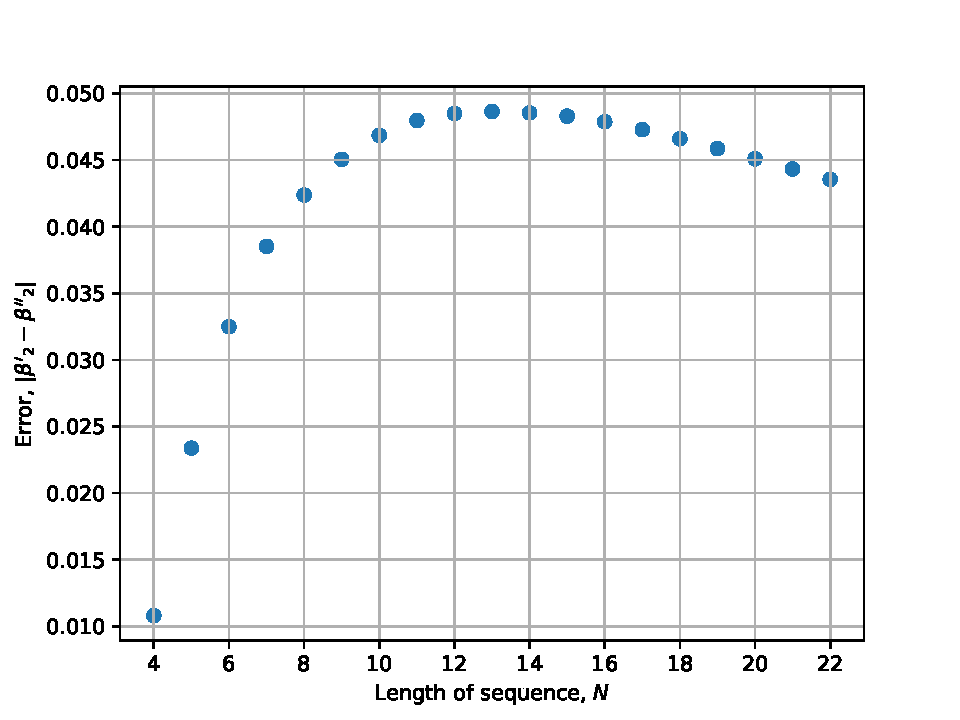
\includegraphics[width=\textwidth]{figs/ch3_QSD/betap_betapp_pi_4_2CP.pdf}
        \caption{Absolute value of the difference between~\eqref{eq:ch3_QSD-reduceddual} and its heuristic.}
    \end{subfigure}
    \hfill
    \begin{subfigure}[b]{0.495\textwidth}
        \centering
        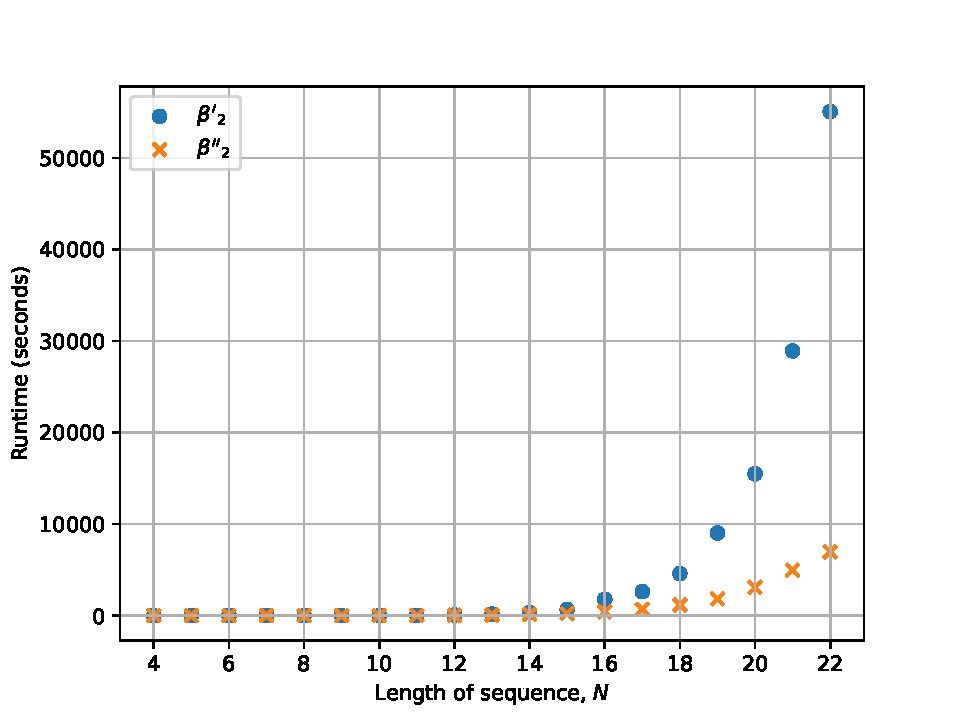
\includegraphics[width=\textwidth]{figs/ch3_QSD/betap_betapp_time_pi_4_2CP.pdf}
        \caption{Runtimes of~\eqref{eq:ch3_QSD-reduceddual} and its heuristic.}
    \end{subfigure}
    \caption{
    Here we look at the case where the state $\ket{0}$ mutated to the state $\ket{+}$ which in turn mutated to the state $\ket{1}$.
    For the reward described in Eq.~\eqref{eq:ch3_QSD-2CP_ctbr}, we depict the error between the heuristic and the solution~\eqref{eq:ch3_QSD-reduceddual} (on the left), as well as the runtimes of both~\eqref{eq:ch3_QSD-reduceddual} and the heuristic (on the right).
    For a short sequence up to length $13$, computing the heuristic might be a disadvantage.
    But for sequences of larger lengths, the heuristic is roughly \emph{eight} times faster than~\eqref{eq:ch3_QSD-reduceddual} with a difference of only about $0.044$ between their computed values.
    To compute~\eqref{eq:ch3_QSD-reduceddual} for sequence of length $22$, it takes about $15$ hours.
    If one were to continue this experiment for larger lengths of sequences, one should expect a behavior similar to Figure~\ref{fig:ch3_QSD-beta'_beta''_pi_4_1CP} (a).
    }
    \label{fig:ch3_QSD-beta'_beta''_pi_4_2CP}
\end{figure}

\section{At most three changepoints}\label{sec:ch3_QSD-3CP}

If we have at most three changepoints, Bob has to consider the following states
\begin{equation}
    \label{eq:ch3_QSD-3CP}
    \begin{aligned}
        \ket{\tau_{c_1 c_2 c_3}} &\coloneqq \ket{\tau_{c_1 c_2 c_3 N \cdots N}} = \ket{\psi}^{\otimes c_1}\ \otimes \ket{\phi_1}^{\otimes (c_2 - c_1)}\ \otimes \ket{\phi_2}^{\otimes (c_3 - c_2)}\ \otimes \ket{\phi_3}^{\otimes (N - c_3)}, \quad (c_1, c_2, c_3) \in \Iset_N.
    \end{aligned}
\end{equation}
Note here that
\begin{align}
    \ket{\tau_{c_1 c_2}} \coloneqq \ket{\tau_{c_1 c_2 N}} = \ket{\psi}^{\otimes c_1}\ \otimes \ket{\phi_1}^{\otimes (c_2 - c_1)}\ \otimes \ket{\phi_2}^{\otimes (N - c_2)}
\end{align}
is the sequence for at most two changepoints,
\begin{align}
    \ket{\tau_{c_1}} \coloneqq \ket{\tau_{c_1 N N}} = \ket{\psi}^{\otimes c_1}\ \otimes \ket{\phi_1}^{\otimes (N - c_1)}
\end{align}
denotes the sequences corresponding to a single changepoint and
\begin{align}
    \ket{\tau_N} \coloneqq \ket{\tau_{N N N}} = \ket{\psi}^{\otimes N} 
\end{align}
indicates the sequence with no changepoint.

\paragraph{Gram matrix.}

\begin{align}
    T_{ijk,lmn} =
    \begin{cases}
        \gamma_1^{|i-l|}\ \gamma_{12}^{|j-k|}\ \gamma_{13}^{|k-m|} \gamma_{23}^{|m-n|},\ \hspace{30pt} l \le j \le k \le m \\
        \gamma_1^{|i-l|}\ \gamma_{12}^{|j-m|}\ \gamma_{23}^{|k-n|},\ \hspace{60pt} l \le j \le n \text{ and } k > m \\
        \gamma_1^{|i-l|}\ \gamma_{12}^{|m-n|}\ \gamma_{13}^{|n-j|},\ \hspace{60pt} l \le m \le n < j \le k \\
        \gamma_1^{|i-j|}\ \gamma_2^{|j-l|}\ \gamma_{12}^{|l-k|}\ \gamma_{13}^{|k-m|}\ \gamma_{23}^{|m-n|},\ j < l \le k \le m \\
        \gamma_1^{|i-j|}\ \gamma_2^{|j-l|}\ \gamma_{12}^{|l-m|},\ \hspace{62pt} j < l \le k \text{ and } k > m \\
        \gamma_1^{|i-j|}\ \gamma_2^{|j-k|}\ \gamma_3^{|k-l|}\ \gamma_{13}^{|l-m|}\ \gamma_{23}^{|m-n|},\ j \le k < l
    \end{cases}. 
\end{align}

In this formula, we assume that $i \le l$.
It is straightforward to compute the other entries since the block matrix is symmetric.

The Gram matrix can be depicted as the block matrix denoted in Eq.~(\ref{eq:ch3_QSD-T_3CP}).
\begin{align}
    \label{eq:ch3_QSD-T_3CP}
    T_{3CP} =
    \begin{pmatrix}
        V_{11} & V_{12} & V_{13} & \cdots & V_{1,N-2} & V_{1,N-1} & \rvline & V_{1N} \\
        V_{12}^\top & V_{11}^{[1]} & V_{12}^{[1]} & \cdots & V_{1,N-3}^{[1]} & V_{1,N-2}^{[1]} & \rvline & V_{2N} \\
        V_{13}^\top & V_{12}^{[1]\top} & V_{11}^{[2]} & \cdots & V_{1,N-4}^{[2]} & V_{1, N-3}^{[2]} & \rvline & V_{3N} \\
        \vdots & \vdots & \vdots & \ddots & \vdots & \vdots & \rvline & \vdots \\
        V_{1,N-2}^\top & V_{1,N-3}^{[1]\top} & V_{1,N-4}^{[2]\top} & \cdots & V_{11}^{[N-3]} & V_{12}^{[N-3]} & \rvline & V_{N-2,N} \\
        V_{1,N-1}^\top & V_{1,N-2}^{[1]\top} & V_{1,N-3}^{[2]\top} & \cdots & V_{12}^{[N-3]\top} & V_{11}^{[N-2]} & \rvline & V_{N-1,N} \\
        \hline
        V_{1N}^\top & V_{2N}^\top & V_{3N}^\top & \cdots & V_{N-2,N}^\top & V_{N-1,N}^\top & \rvline & 1 \\
    \end{pmatrix}. 
\end{align}
Each block $V_{ik}$ is a matrix containing $(N-i) \times (N-k)$ blocks.
The notation $V_{ik}^{[m]}$ indicates the block matrix obtained by discarding the blocks along the \emph{first} $m$ rows and the \emph{first} $m$ columns of $V_{ik}$.

Determining the matrices along the \emph{first} row and the \emph{last} column of $T_{3CP}$ is sufficient to construct the entire matrix.
Eqs.~\eqref{eq:ch3_QSD-V_11}-\eqref{eq:ch3_QSD-V_2N} describe how to construct each of the matrices $V_{1k}$ and $V_{iN}$ for $i, k \in \{1, \dots, N-1\}$.
Each block in this block matrix $S_{ij,kl}$ is constructed in the same manner as was used by $T_{ik}$ in Section~\ref{sec:ch3_QSD-2CP}.
The matrix $S_{12,12}$ is symmetric Toeplitz where each entry is given as $(S_{12,12})_{jl} = \gamma_{23}^{|j-l|}$.
We therefore have the following matrices

\begin{align}
    \label{eq:ch3_QSD-V_11}
    V_{11} =
    \begin{pmatrix}
        S_{12,12} & S_{12,13} & S_{12,14} & \cdots & S_{12,1,N-2} & S_{12,1,N-1} & \rvline & S_{12,1N} \\
        S_{12,13}^\top & S_{12,12}^{(1)} & S_{12,13}^{(1)} & \cdots & S_{12,1,N-3}^{(1)} & S_{12,1,N-2}^{(1)} & \rvline & S_{13,1N} \\
        S_{12,14}^\top & S_{12,13}^{(1)\top} & S_{12,12}^{(2)} & \cdots & S_{12,1,N-4}^{(2)} & S_{12,1,N-3}^{(2)} & \rvline & S_{14,1N} \\
        \vdots & \vdots & \vdots & \ddots & \vdots & \vdots & \rvline & \vdots \\
        S_{12,1,N-2}^\top & S_{12,1,N-3}^{(1)\top} & S_{12,1,N-4}^{(2)\top} & \cdots & S_{12,12}^{(N-4)} & S_{12,13}^{(N-4)} & \rvline & S_{1,N-2,1N} \\
        S_{12,1,N-1}^\top & S_{12,1,N-2}^{(1)\top} & S_{12,1,N-3}^{(2)\top} & \cdots & S_{12,13}^{(N-4)\top} & S_{12,12}^{(N-3)} & \rvline & S_{1,N-1,1N} \\
        \hline
        S_{12,1N}^\top & S_{13,1N}^\top & S_{14,1N}^\top & \cdots & S_{1,N-2,1N}^\top & S_{1,N-1,1N} & \rvline & 1 \\
    \end{pmatrix}
\end{align}

\begin{align}
    \label{eq:ch3_QSD-V_12}
    V_{12} =
    \begin{pmatrix}
        S_{12,23} & S_{12,24} & S_{12,25} & \cdots & S_{12,2,N-2} & S_{12,2,N-1} & \rvline & S_{12,2N} \\
        S_{13,23} & S_{12,23}^{(1)} & S_{12,24}^{(1)} & \cdots & S_{12,2,N-3}^{(1)} & S_{12,2,N-2}^{(1)} & \rvline & S_{13,2N} \\
        S_{12,23}^{(1)\top} & S_{13,23}^{(1)} & S_{12,23}^{(2)} & \cdots & S_{12,2,N-4}^{(2)} & S_{12,2,N-3}^{(2)} & \rvline & S_{14,2N} \\
        \vdots & \vdots & \vdots & \ddots & \vdots & \vdots & \rvline & \vdots \\
        S_{12,2,N-3}^{(1)\top} & S_{12,2,N-4}^{(2)\top} & S_{12,2,N-5}^{(2)\top} & \cdots & S_{13,23}^{(N-5)} & S_{12,23}^{(N-5)} & \rvline & S_{1,N-2,2N} \\
        S_{12,2,N-2}^{(1)\top} & S_{12,2,N-3}^{(2)\top} & S_{12,2,N-4}^{(2)\top} & \cdots & S_{12,23}^{(N-5)\top} & S_{13,23}^{(N-4)} & \rvline & S_{1,N-1,2N} \\
        \hline
        S_{13,2N}^\top & S_{14,2N}^\top & S_{15,2N}^\top & \cdots & S_{1,N-2,2N}^\top & S_{1,N-1,2N}^\top & \rvline & S_{1N,2N}
    \end{pmatrix}
\end{align}

\begin{align}
    \label{eq:ch3_QSD-V_13}
    V_{13} = 
    \begin{pmatrix}
        S_{12,34} & S_{12,35} & S_{12,36} & \cdots & S_{12,3,N-2} & S_{12,3,N-1} & \rvline & S_{12,3N} \\
        S_{13,34} & S_{12,34}^{(1)} & S_{12,35}^{(1)} & \cdots & S_{12,3,N-3}^{(1)} & S_{12,3,N-2}^{(1)} & \rvline & S_{13,3N} \\
        S_{14,34} & S_{13,34}^{(1)} & S_{12,34}^{(1)} & \cdots & S_{12,3,N-4}^{(2)} & S_{12,3,N-3}^{(2)} & \rvline & S_{14,3N} \\
        \vdots & \vdots & \vdots & \ddots & \vdots & \vdots & \rvline & \vdots \\
        S_{12,3,N-4}^{(2)\top} & S_{12,3,N-5}^{(3)\top} & S_{12,3,N-6}^{(4)\top} & \cdots & S_{14,34}^{(N-6)} & S_{13,34}^{(N-6)} & \rvline & S_{1,N-2,3N} \\
        S_{12,3,N-3}^{(2)\top} & S_{12,3,N-4}^{(3)\top} & S_{12,3,N-5}^{(4)\top} & \cdots & S_{13,34}^{(N-6)\top} & S_{14,34}^{(N-5)} & \rvline & S_{1,N-1,3N} \\
        \hline
        S_{14,3N}^\top & S_{15,3N}^\top & S_{16,3N}^\top & \cdots & S_{1,N-2,3N}^\top & S_{1,N-1,3N}^\top & \rvline & S_{1N,3N}
    \end{pmatrix}
\end{align}

\begin{align}
    \label{eq:ch3_QSD-V_1N_2}
    V_{1,N-2} =
    \begin{pmatrix}
        S_{12,N-2,N-1} & \rvline & S_{12,N-2,N} \\
        S_{13,N-2,N-1} & \rvline & S_{13,N-2,N} \\
        S_{14,N-2,N-1} & \rvline & S_{14,N-2,N} \\
        \vdots & \rvline & \vdots \\
        S_{1,N-2,N-2,N-1} & \rvline & S_{1,N-2,N-2,N} \\
        S_{1,N-1,N-2,N-1} & \rvline & S_{1,N-1,N-2,N} \\
        S_{1N,N-2,N-1} & \rvline & S_{1N,N-2,N} \\
    \end{pmatrix}
    \quad
    V_{1,N-1} = 
    \begin{pmatrix}
        S_{12,N-1,N} \\
        S_{13,N-1,N} \\
        S_{14,N-1,N} \\
        \vdots \\
        S_{1,N-2,N-1,N} \\
        S_{1,N-1,N-1,N} \\
        S_{1N,N-1,N} \\
    \end{pmatrix}
    \quad
    V_{1N} =
    \begin{pmatrix}
        S_{12,NN} \\
        S_{13,NN} \\
        S_{14,NN} \\
        \vdots \\
        S_{1,N-2,NN} \\
        S_{1,N-1,NN} \\
        S_{1N,NN} \\
    \end{pmatrix}
\end{align}

\begin{align}
    \label{eq:ch3_QSD-V_2N}
    V_{2N} =
    \begin{pmatrix}
        S_{23,NN} \\
        S_{24,NN} \\
        \vdots \\
        S_{2,N-2,NN} \\
        S_{2,N-1,NN} \\
        S_{2N,NN} \\
    \end{pmatrix},
    \
    V_{3N} =
    \begin{pmatrix}
        S_{34,NN} \\
        \vdots \\
        S_{3,N-2,NN} \\
        S_{3,N-1,NN} \\
        S_{3N,NN} \\
    \end{pmatrix},
    \
    V_{N-2,N} =
    \begin{pmatrix}
        S_{N-2,N-1,NN} \\
        S_{N-2,N,NN}
    \end{pmatrix},
    \
    V_{N-1,N} =
    \begin{pmatrix}
        S_{N-1,N,NN}
    \end{pmatrix}.
\end{align}

\paragraph{Heuristic approach.}

We once again exploit the Toeplitz-like structure of the Gram matrix and restrict the solution $X_{3CP}$ to have a similar structure as below
\begin{align}
    \label{eq:ch3_QSD-X_3CP}
    X'_{3CP} =
    \begin{pmatrix}
        Y_{11} & Y_{12} & Y_{13} & \cdots & Y_{1,N-2} & Y_{1,N-1} & \rvline & \\
        Y_{12}^\top & Y_{11}^{[1]} & Y_{12}^{[1]} & \cdots & Y_{1,N-3}^{[1]} & Y_{1,N-2}^{[1]} & \rvline & \\
        Y_{13}^\top & Y_{12}^{[1]\top} & Y_{11}^{[2]} & \cdots & Y_{1,N-4}^{[2]} & Y_{1,N-3}^{[2]} & \rvline \\
        \vdots & \vdots & \vdots & \ddots & \vdots & \vdots & \rvline & y_N \\
        Y_{1,N-2}^\top & Y_{1,N-3}^{[1]\top} & Y_{1,N-4}^{[2]\top} & \cdots & Y_{11}^{[N-3]} & Y_{12}^{[N-3]} & \rvline & \\
        Y_{1,N-1}^\top & Y_{1,N-2}^{[1]\top} & Y_{1,N-3}^{[2]\top} & \cdots & Y_{12}^{[N-3]\top} & Y_{11}^{[N-2]} & \rvline & \\
        \hline
         &  &  & y_N^\top &  &  & \rvline & z \\
    \end{pmatrix}
\end{align}

\begin{align}
    \label{eq:ch3_QSD-Y_11}
    Y_{11} =
    \begin{pmatrix}
        W_{12,12} & W_{12,13} & W_{12,14} & \cdots & W_{12,1,N-2} & W_{12,1,N-1} & \rvline & \\
        W_{12,13}^\top & W_{12,12}^{(1)} & W_{12,13}^{(1)} & \cdots & W_{12,1,N-3}^{(1)} & W_{12,1,N-2}^{(1)} & \rvline & \\
        W_{12,14}^\top & W_{12,13}^{(1)\top} & W_{12,12}^{(2)} & \cdots & W_{12,1,N-4}^{(2)} & W_{12,1,N-3}^{(2)} & \rvline & \\
        \vdots & \vdots & \vdots & \ddots & \vdots & \vdots & \rvline & w_{1N} \\
        W_{12,1,N-2}^\top & W_{12,1,N-3}^{(1)\top} & W_{12,1,N-4}^{(2)\top} & \cdots & W_{12,12}^{(N-4)} & W_{12,13}^{(N-4)} & \rvline & \\
        W_{12,1,N-1}^\top & W_{12,1,N-2}^{(1)\top} & W_{12,1,N-3}^{(2)\top} & \cdots & W_{12,13}^{(N-4)\top} & W_{12,12}^{(N-3)} & \rvline & \\
        \hline
         &  &  & w_{1N}^\top &  &  & \rvline & z_{1N} \\
    \end{pmatrix}
\end{align}

\begin{align}
    \label{eq:ch3_QSD-Y_12}
    Y_{12} =
    \begin{pmatrix}
        W_{12,23} & W_{12,24} & W_{12,25} & \cdots & W_{12,2,N-2} & W_{12,2,N-1} & \rvline & \\
        W_{13,23} & W_{12,23}^{(1)} & W_{12,24}^{(1)} & \cdots & W_{12,2,N-3}^{(1)} & W_{12,2,N-2}^{(1)} & \rvline &  \\
        W_{12,23}^{(1)\top} & W_{13,23}^{(1)} & W_{12,23}^{(2)} & \cdots & W_{12,2,N-4}^{(2)} & W_{12,2,N-3}^{(2)} & \rvline &  \\
        \vdots & \vdots & \vdots & \ddots & \vdots & \vdots & \rvline & w_{2N} \\
        W_{12,2,N-3}^{(1)\top} & W_{12,2,N-4}^{(2)\top} & W_{12,2,N-5}^{(2)\top} & \cdots & W_{13,23}^{(N-5)} & W_{12,23}^{(N-4)} & \rvline &  \\
        W_{12,2,N-2}^{(1)\top} & W_{12,2,N-3}^{(2)\top} & W_{12,2,N-4}^{(2)\top} & \cdots & W_{12,23}^{(N-4)\top} & W_{13,23}^{(N-4)} & \rvline &  \\
        \hline
         &  &  & w_{2N}^\top &  &  & \rvline & z_{2N} \\
    \end{pmatrix}
\end{align}

\begin{align}
    \label{eq:ch3_QSD-Y_13}
    Y_{13} =
    \begin{pmatrix}
        W_{12,34} & W_{12,35} & W_{12,36} & \cdots & W_{12,3,N-2} & W_{12,3,N-1} & \rvline &  \\
        W_{13,34} & W_{12,34}^{(1)} & W_{12,35}^{(1)} & \cdots & W_{12,3,N-3}^{(1)} & W_{12,3,N-2}^{(1)} & \rvline &  \\
        W_{14,34} & W_{13,34}^{(1)} & W_{12,34}^{(1)} & \cdots & W_{12,3,N-4}^{(2)} & W_{12,3,N-3}^{(2)} & \rvline &  \\
        \vdots & \vdots & \vdots & \ddots & \vdots & \vdots & \rvline & w_{3N} \\
        W_{12,3,N-4}^{(2)\top} & W_{12,3,N-5}^{(3)\top} & W_{12,3,N-6}^{(4)\top} & \cdots & W_{14,34}^{(N-6)} & W_{13,34}^{(N-6)} & \rvline &  \\
        W_{12,3,N-3}^{(2)\top} & W_{12,3,N-4}^{(3)\top} & W_{12,3,N-5}^{(4)\top} & \cdots & W_{13,34}^{(N-6)\top} & W_{14,34}^{(N-5)} & \rvline &  \\
        \hline
         &  &  & w_{3N}^\top &  &  & \rvline & z_{3N}
    \end{pmatrix}
\end{align}

\begin{align}
    \label{eq:ch3_QSD-Y_1N_2}
    Y_{1,N-2} =
    \begin{pmatrix}
        W_{12,N-2,N-1} & \rvline &  \\
        W_{13,N-2,N-1} & \rvline &  \\
        W_{14,N-2,N-1} & \rvline &  \\
        \vdots & \rvline & w_{N-2,N} \\
        W_{1,N-2,N-2,N-1} & \rvline &  \\
        W_{1,N-1,N-2,N-1} & \rvline &  \\
        W_{1N,N-2,N-1} & \rvline &  \\
    \end{pmatrix},
\end{align}

where $Y_{1,N-1}$ is a vector of size $N-1$, while $y_N$ is a vector of size $N + \frac{N (N-1) (N-2)}{6}$.

Finally, we consider all the possible sequential mutations, $\ket{0}$ to $\ket{+}$, $\ket{+}$ to $\ket{1}$, and $\ket{1}$ to $-\ket{-}$.
In other words, Bob must discriminate between all the possible states described in Eq.~(\eqref{eq:ch3_QSD-no_CP_eg}, \eqref{eq:ch3_QSD-1CP_eg}, \eqref{eq:ch3_QSD-2CP_eg}, \ref{eq:ch3_QSD-3CP_eg}).

The reward strategy in accordance with the closer-the better rewards in Eq.~\eqref{eq:ch3_QSD-R_ME_SD} is
\begin{align}
    \label{eq:ch3_QSD-3CP_ctbr}
    R_{fgh, ijk} =
    \begin{cases}
        0, & f = N+1 \\
        \left( \frac{1}{\sqrt{2}} \right)^{|f-i|} \left( \frac{1}{\sqrt{2}} \right)^{|g-h|} \left( \frac{1}{\sqrt{2}} \right)^{|j-k|}, & f \ne N+1,\ i \le g \le h \le j \\
        \left( \frac{1}{\sqrt{2}} \right)^{|f-i|} \left( \frac{1}{\sqrt{2}} \right)^{|g-j|} \left( \frac{1}{\sqrt{2}} \right)^{|h-k|}, & f \ne N+1,\ i \le g \le k \text{ and } h > j \\
        \left( \frac{1}{\sqrt{2}} \right)^{|f-i|} \left( \frac{1}{\sqrt{2}} \right)^{|j-k|}, & f \ne N+1,\ i \le j \le k < g \le h \\
        \left( \frac{1}{\sqrt{2}} \right)^{|f-g|} \left( \frac{1}{\sqrt{2}} \right)^{|i-h|} \left( \frac{1}{\sqrt{2}} \right)^{|j-k|}, & f \ne N+1,\ g < i \le h \le j \\
        \left( \frac{1}{\sqrt{2}} \right)^{|f-g|} \left( \frac{1}{\sqrt{2}} \right)^{|i-j|}, & f \ne N+1,\ g < i \le h \text{ and } h > j \\
        \left( \frac{1}{\sqrt{2}} \right)^{|f-g|} \left( \frac{1}{\sqrt{2}} \right)^{|h-i|} \left( \frac{1}{\sqrt{2}} \right)^{|j-k|}, & f \ne N+1,\ g \le h < i
    \end{cases}. 
\end{align}

Figure~\ref{fig:ch3_QSD-beta'_beta''_pi_4_3CP} compares the runtime and the absolute difference in the solutions of the reduced SDP~\eqref{eq:ch3_QSD-reduceddual} when the variable $X$ is constrained to be Hermitian, and the heuristic when the variable $X$ is constrained to satisfy Eq.~\eqref{eq:ch3_QSD-X_3CP}, as a function of the length of the sequence $N$.
Note here that for sequence of length $12$, solving~\eqref{eq:ch3_QSD-reduceddual} involves computing a matrix of size $4096 \times 4096$.
Up to a sequence of length $8$, there is no gain in the runtime when computing the heuristic.
As $N$ gets larger, the heuristic is about \emph{ten} times faster than~\eqref{eq:ch3_QSD-reduceddual} (on the right) with an error of roughly $0.083$ for $N = 12$.

\begin{figure}[htb]
    \centering
    \begin{subfigure}[b]{0.495\textwidth}
        \centering
        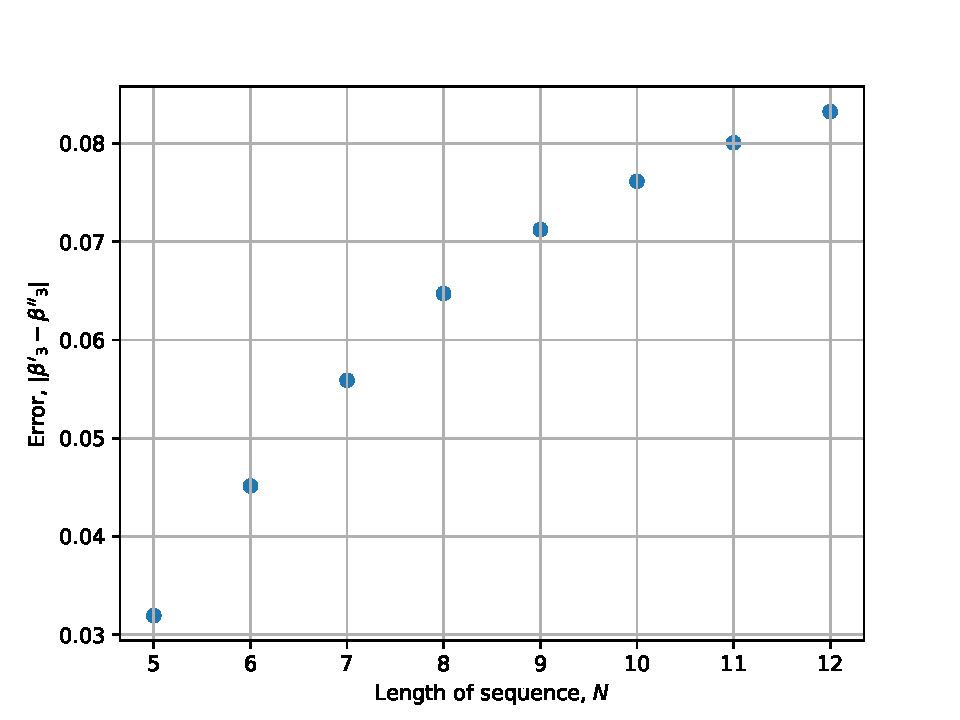
\includegraphics[width=\textwidth]{figs/ch3_QSD/betap_betapp_pi_4_3CP.pdf}
        \caption{Absolute value of the difference between Eq.~\eqref{eq:ch3_QSD-reduceddual} and its heuristic.}
    \end{subfigure}
    \hfill
    \begin{subfigure}[b]{0.495\textwidth}
        \centering
        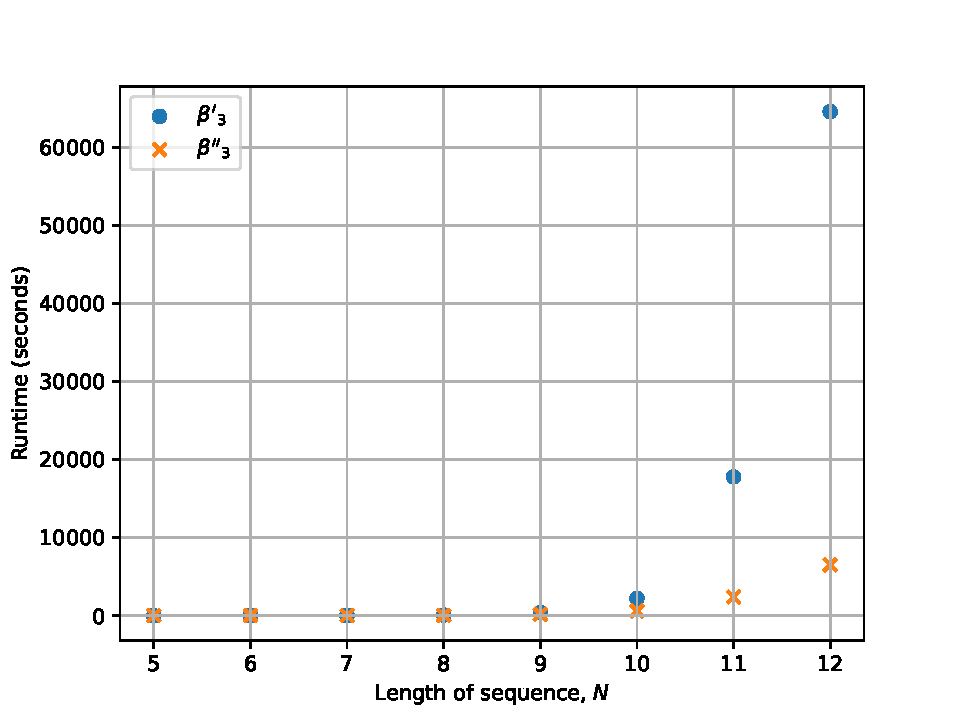
\includegraphics[width=\textwidth]{figs/ch3_QSD/betap_betapp_time_pi_4_3CP.pdf}
        \caption{Runtimes of Eq.~\eqref{eq:ch3_QSD-reduceddual} and its heuristic.}
    \end{subfigure}
    \caption{
    We look at sequences with three changepoints, each being sequences of $N$ states starting at $\ket{0}$ and first switching to $\ket{+}$, then to $\ket{1}$, and finally to $-\ket{-}$.
    Under the reward function of Eq.~\eqref{eq:ch3_QSD-3CP_ctbr}, we see the error (on the left) and the runtime (on the right) of both the solution~\eqref{eq:ch3_QSD-reduceddual} and the heuristic.
    The SDP solving this heuristic is of size $\Ocomp(N^3)$.
    Comparing the runtimes we see that up to a sequence of $8$, there is no gain in the runtime by computing the heuristic.
    Beyond this, the heuristic is about \emph{ten} times faster than~\eqref{eq:ch3_QSD-reduceddual} (on the right) with an error of roughly $0.083$ for $N = 12$.
    We terminate execution at $N = 12$ because computing~\eqref{eq:ch3_QSD-reduceddual} takes $18$ hours.
    It would be reasonable to assume that for larger sequences, the error will resemble that of the one changepoint case illustrated in Figure~\ref{fig:ch3_QSD-beta'_beta''_pi_4_1CP} (a).
    }
    \label{fig:ch3_QSD-beta'_beta''_pi_4_3CP}
\end{figure}

We consider the previous discussion replacing these states $\ket{0}, \ket{+}, \ket{1}$ and $-\ket{-}$ with qubits differing by an angle of $\theta$ (Eq.~\eqref{eq:ch3_QSD-theta_states}) instead, in the next section. 
%Section~\ref{sec:ch3_QSD-theta_expts}.

\begin{comment}
\subsection{Multiple changepoint problem} \label{sec:ch3_QSD-MCP} 

We now consider the scenario where Alice promises $n$ copies of the state $\ket{0}$, but there are a total of three changepoints; starting from $\ket{0}$ and eventually possibly changing to $\ket{+}$, to $\ket{1}$, and to $-\ket{-}$, in that order.
Figure~\ref{fig:ch3_QSD-beta'_beta''_pi_4_3CP} (a) and Figure~\ref{fig:ch3_QSD-beta'_beta''_pi_4_3CP} (b) compare the error and their runtimes of the reduced dual \eqref{eq:ch3_QSD-reduceddual} and the heuristic \eqref{eq:ch3_QSD-T_3CP} respectively.
These examples and more are described in further detail in Section~\ref{sec:ch3_QSD-expts}.

\begin{figure}[h]
    \centering
    \begin{subfigure}[b]{0.495\textwidth}
        \centering
        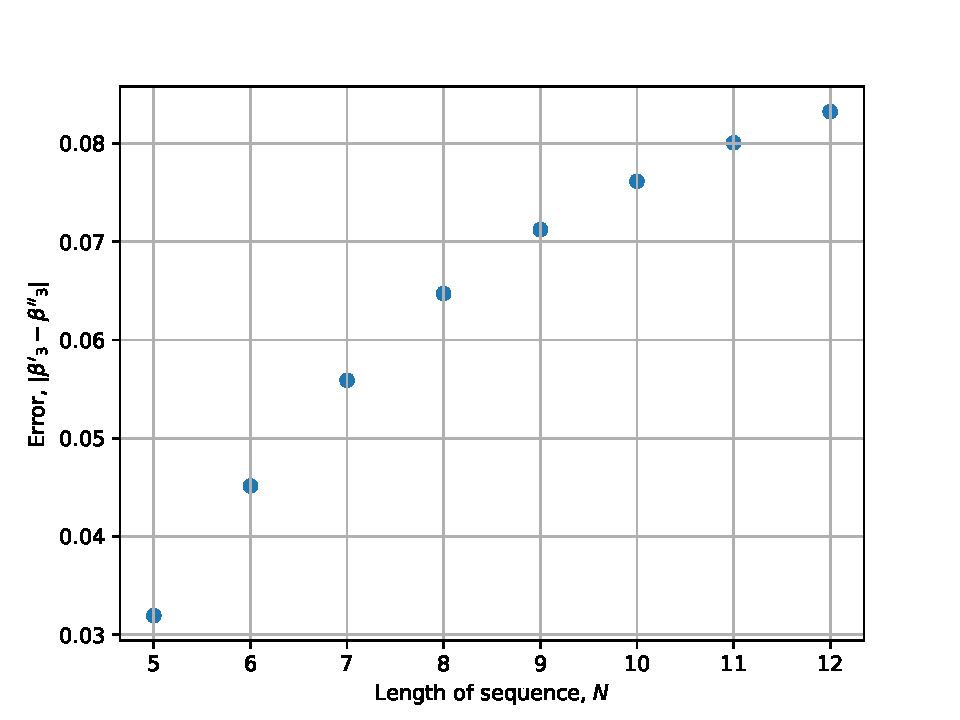
\includegraphics[width=\textwidth]{figs/ch3_QSD/betap_betapp_pi_4_3CP.pdf}
        \caption{Absolute value of the difference between \eqref{eq:ch3_QSD-reduceddual} and \eqref{eq:ch3_QSD-T_3CP}.}
    \end{subfigure}
    \hfill
    \begin{subfigure}[b]{0.495\textwidth}
        \centering
        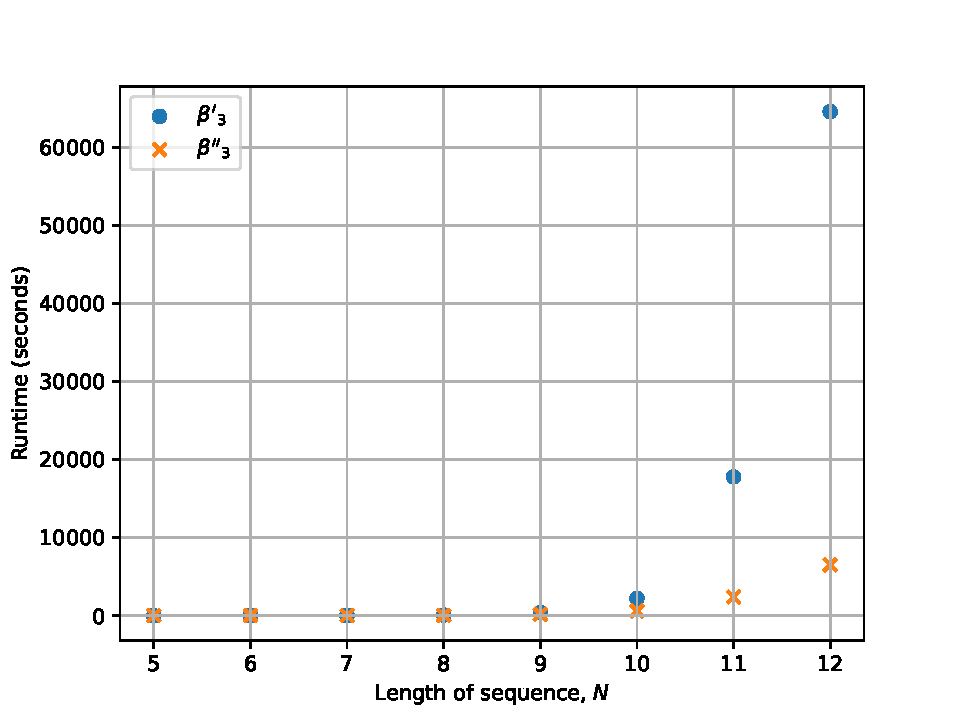
\includegraphics[width=\textwidth]{figs/ch3_QSD/betap_betapp_time_pi_4_3CP.pdf}
        \caption{Runtimes of \eqref{eq:ch3_QSD-reduceddual} and \eqref{eq:ch3_QSD-T_3CP}.}
    \end{subfigure}
    \caption{
    We examine the sequences with three changepoints, each of $N$ states, starting at $\ket{0}$, then mutating to $\ket{+}$, to $\ket{1}$ and $-\ket{-}$, in that order.
    Here we consider a closer-the-better reward structure (discussed in Section~\ref{sec:ch3_QSD-expts}).
    Under this reward scheme, we see the error (on the left) and the runtime (on the right) of both \eqref{eq:ch3_QSD-reduceddual} and the heuristic (\eqref{eq:ch3_QSD-T_3CP}, discussed in Section~\ref{sec:ch3_QSD-expts}).
    We would like to note that the SDP variable size to solve \eqref{eq:ch3_QSD-reduceddual} is of size $\Ocomp(N^3)$.
    There is an error of roughly $0.083$ for the sequence of length $12$.
    At this sequence length, \eqref{eq:ch3_QSD-T_3CP} is about \emph{ten} times faster than \eqref{eq:ch3_QSD-reduceddual}.
    We suspect that for a larger sequence, we will observe a behavior similar to Figure~\ref{fig:ch3_QSD-beta'_beta''_pi_4_1CP_intro} (a).
    However since it takes roughly $18$ hours to compute \eqref{eq:ch3_QSD-reduceddual} for $N = 10$, we are unable to easily test for larger sequences of $N$.
    }
    \label{fig:ch3_QSD-beta'_beta''_pi_4_3CP_intro}
\end{figure} 

In this appendix we describe the scenarios for at most two and three changepoints. 
\end{comment}

%%%%%%%%%%%%%%%%%%%%%%%%%%%%%%%%%%%%%%%%%%%%%%%%%%%%%%%%%%%%%%%%%%%%%%%%%%%%%%%%%%%%%%%%%%%%%%%%%%%%%%%%%%%%%%%%%%%%%%%%%%%%%%%%%%%

\section{At most $p$ changepoints}

Observe that $T_{11}$ in Eq.~\eqref{eq:ch3_QSD-T_2CP} is constructed in the exact same manner as $T_{1CP}$ used in the one changepoint case.
Similarly, $V_{11}$ in Eq.~\eqref{eq:ch3_QSD-T_3CP} follows the same construction as $T_{2CP}$ described in Eq.~\eqref{eq:ch3_QSD-T_2CP}.
Therefore, we guess that a heuristic solution $X'$ to solve the general case can be constructed by exploiting the structure of the corresponding Gram matrix in a similar manner as the cases we examined.

%%%%%%%%%%%%%%%%%%%%%%%%%%%%%%%%%%%%%%%%%%%%%%%%%%%%%%%%%%%%%%%%%%%%%%%%%%%%%%%%%%%%%%%%%%%%%%%%%%%%%%%%%%%%%%%%%%%%%%%%%%%%%%%%%%

\section{Changepoints with varying overlaps}\label{sec:ch3_QSD-theta_expts}

\begin{comment}
We reproduce some of the numerical experiments in Section~\ref{sec:ch3_QSD-expts} with states differing by an angle $\theta$ (Section~\ref{sec:ch3_QSD-expts} considered $\theta = \pi/4$).
Note that the rewards also change from $1/\sqrt{2}$ to $\cos(\theta)$ in Eqs.~(\eqref{eq:ch3_QSD-1CP_ctbr}, \eqref{eq:ch3_QSD-2CP_ctbr}, \eqref{eq:ch3_QSD-3CP_ctbr}).
\end{comment}

Note that with the states differing by an angle $\theta$ (other than $\theta = \pi/4$ considered previously), the rewards also change from $1/\sqrt{2}$ to $\cos(\theta)$ in Eqs.~(\eqref{eq:ch3_QSD-1CP_ctbr}, \eqref{eq:ch3_QSD-2CP_ctbr}, \eqref{eq:ch3_QSD-3CP_ctbr}).

Figures~\ref{fig:ch3_QSD-1CP},~\ref{fig:ch3_QSD-2CP} and~\ref{fig:ch3_QSD-3CP} illustrate the optimal reward function and our heuristic for one, two, and three changepoints when $\theta$ takes values in $\{\pi/8,\ \pi/4,\ 3\pi/8\}$.

One thing we note is that the SDP solver is unable to find the solution for the three changepoint scenario when $\theta = \pi/8$ and hence returns an arbitrary value of $-1$ for sequences of length greater than $5$.
Note that even when this occurs, our heuristic approach is able to compute a solution.

A general observation from these figures is that for states that are farther apart, the absolute difference between the heuristic and the solution decreases very rapidly.
As the states get closer to one another, this decrease in the difference happens at a much slower rate.
A possible explanation for this is that when the states are farther apart to begin with, it is not hard to distinguish them as is.
As the length of the sequence increases, the ease of distinguishability also increases.
As the states get closer to one another, the sequence must be fairly large before it becomes easy to distinguish them.

\begin{figure}[h]
    \centering
    \begin{subfigure}[b]{0.495\textwidth}
        \centering
        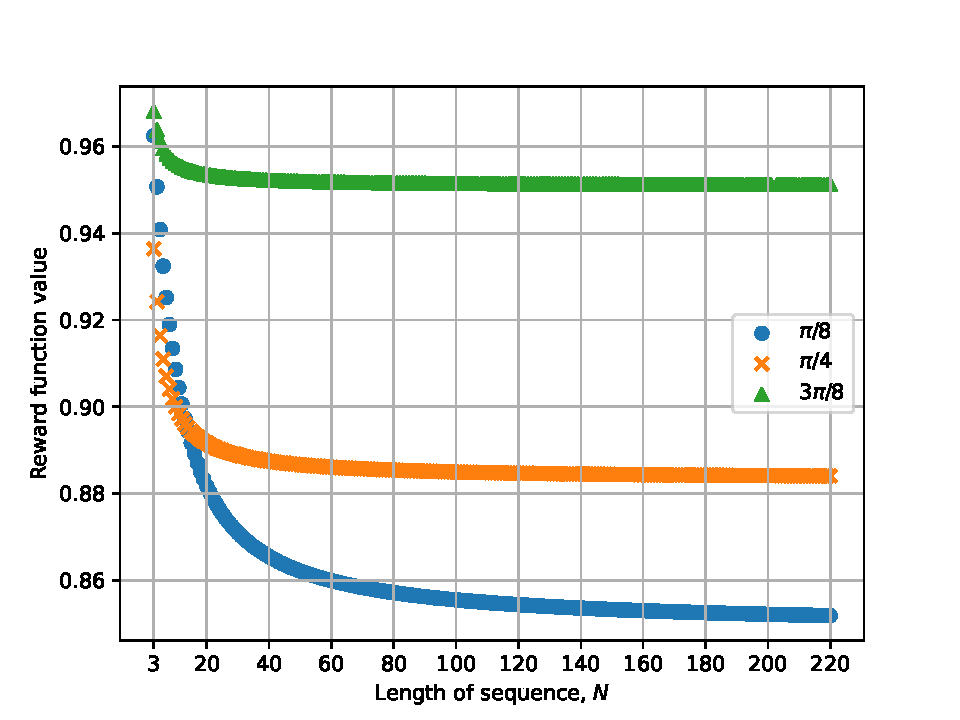
\includegraphics[width=\textwidth]{figs/ch3_QSD/prob_1CP.pdf}
        \caption{Optimal reward function value as a function of $N$ for $\theta \in \{\pi/8, \pi/4, 3\pi/8\}$.}
    \end{subfigure}
    \hfill
    \begin{subfigure}[b]{0.495\textwidth}
        \centering
        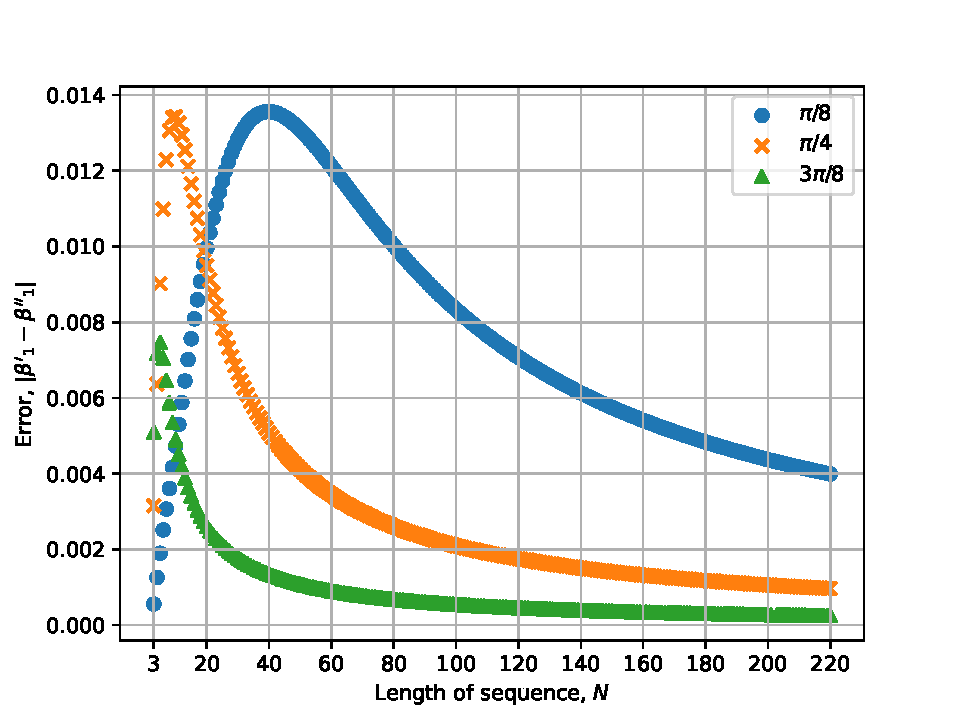
\includegraphics[width=\textwidth]{figs/ch3_QSD/approx_1CP.pdf}
        \caption{Absolute value of the difference between the solution and the heuristic for $\theta \in \{\pi/8, \pi/4, 3\pi/8\}$ as a function of $N$.}
    \end{subfigure}
    \caption{
    Consider the sequences when Alice promises Bob $N$ copies of the state $\ket{0}$ which mutate to the state $\ket{\phi_1} = \cos(\theta) + \sin(\theta)$ for $\theta \in \{\pi/8, \pi/4, 3\pi/8\}$.
    We compare the optimal reward function values for varying $\theta$ as a function of the length of the sequence $N$ (on the left), and the absolute difference between the heuristic and the solution (on the right).
    Observe that for states that are farther apart ($\theta = 3\pi/8$), the error approaches zero rather quickly.
    As the states get closer, it takes much longer for the difference to decrease.
    }
    \label{fig:ch3_QSD-1CP}
\end{figure}

\begin{figure}[h]
    \centering
    \begin{subfigure}[b]{0.495\textwidth}
        \centering
        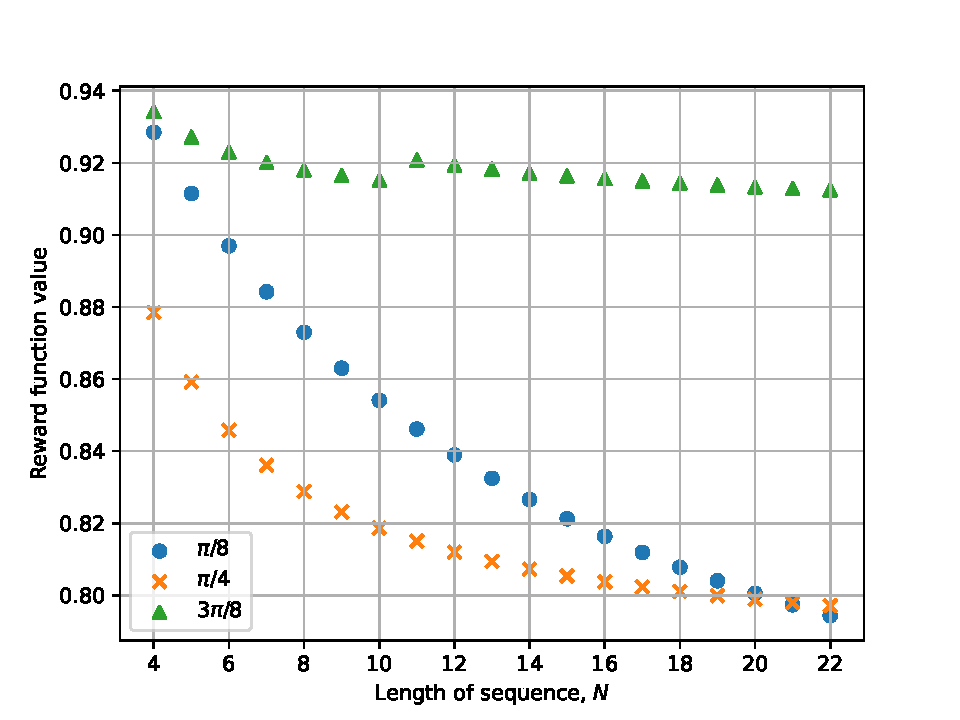
\includegraphics[width=\textwidth]{figs/ch3_QSD/prob_2CP.pdf}
        \caption{Optimal reward function value as a function of $N$ for $\theta \in \{\pi/8, \pi/4, 3\pi/8\}$.}
    \end{subfigure}
    \hfill
    \begin{subfigure}[b]{0.495\textwidth}
        \centering
        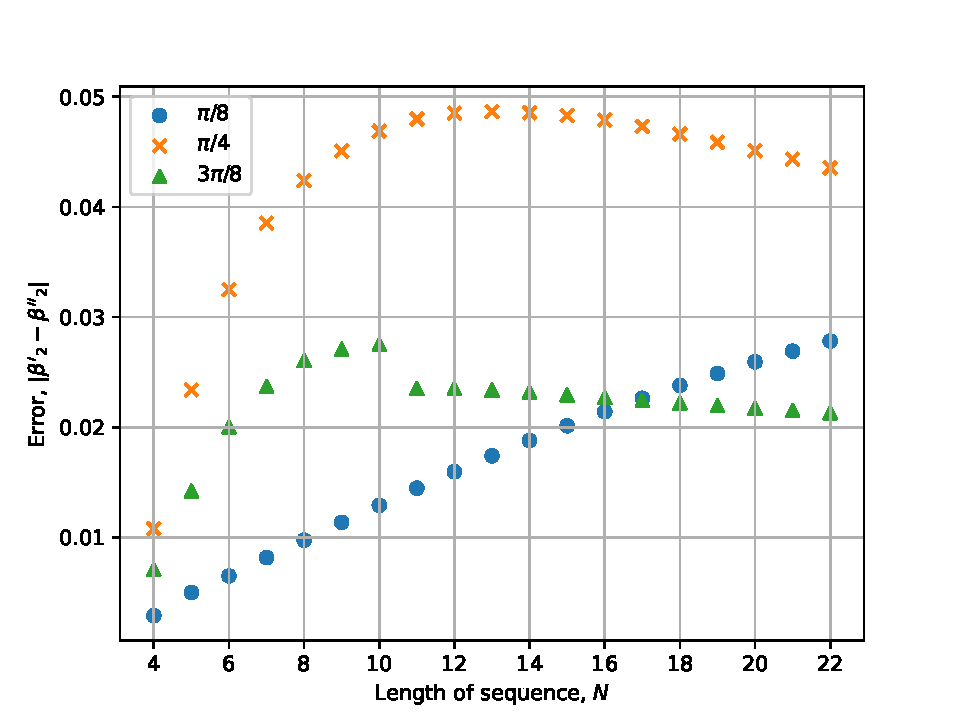
\includegraphics[width=\textwidth]{figs/ch3_QSD/approx_2CP.pdf}
        \caption{Absolute value of the difference between the solution and the heuristic for $\theta \in \{\pi/8, \pi/4, 3\pi/8\}$ as a function of $N$.}
    \end{subfigure}
    \caption{
    Here we consider the scenario where the state $\ket{0}$ first mutates to the state \\ $\ket{\phi_1} = \cos(\theta) + \sin(\theta)$, which further mutates to the state $\ket{\phi_2} = \cos(2\theta) + \sin(2\theta)$, for \\ $\theta \in \{\pi/8, \pi/4, 3\pi/8\}$.
    The optimal reward function values for varying $\theta$ as a function of the length of the sequence $N$ is first compared (on the left), followed by a comparison of the absolute difference between the heuristic and the solution (on the right).
    The behavior is similar to the one changepoint case.
    }
    \label{fig:ch3_QSD-2CP}
\end{figure}

\begin{figure}[h]
    \centering
    \begin{subfigure}[b]{0.495\textwidth}
        \centering
        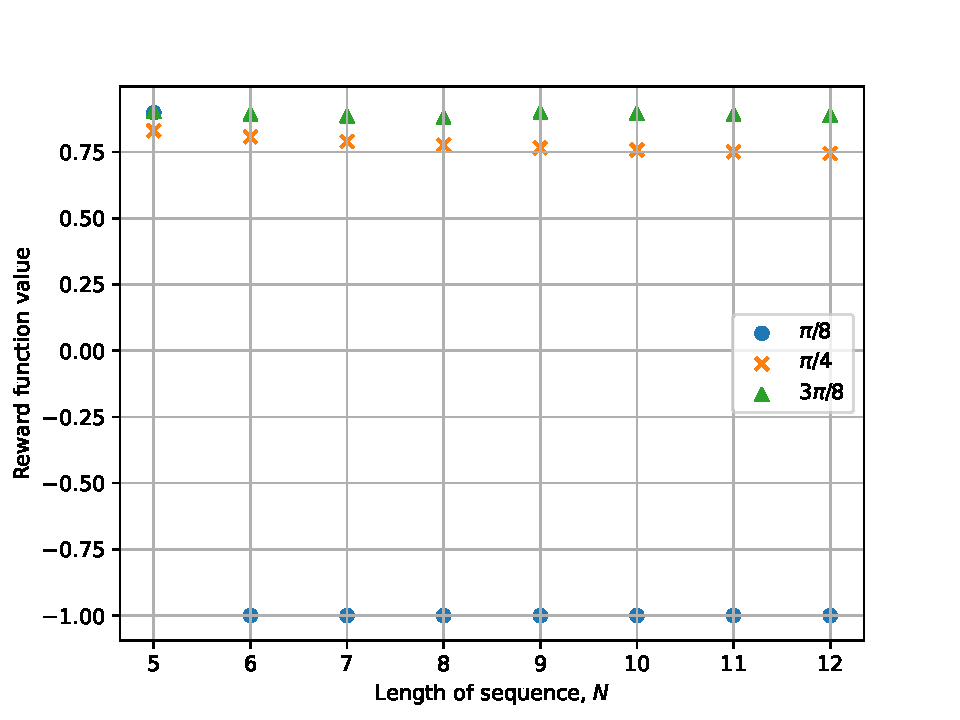
\includegraphics[width=\textwidth]{figs/ch3_QSD/prob_3CP.pdf}
        \caption{Optimal reward function value as a function of $N$ for $\theta \in \{\pi/8, \pi/4, 3\pi/8\}$.}
    \end{subfigure}
    \hfill
    \begin{subfigure}[b]{0.495\textwidth}
        \centering
        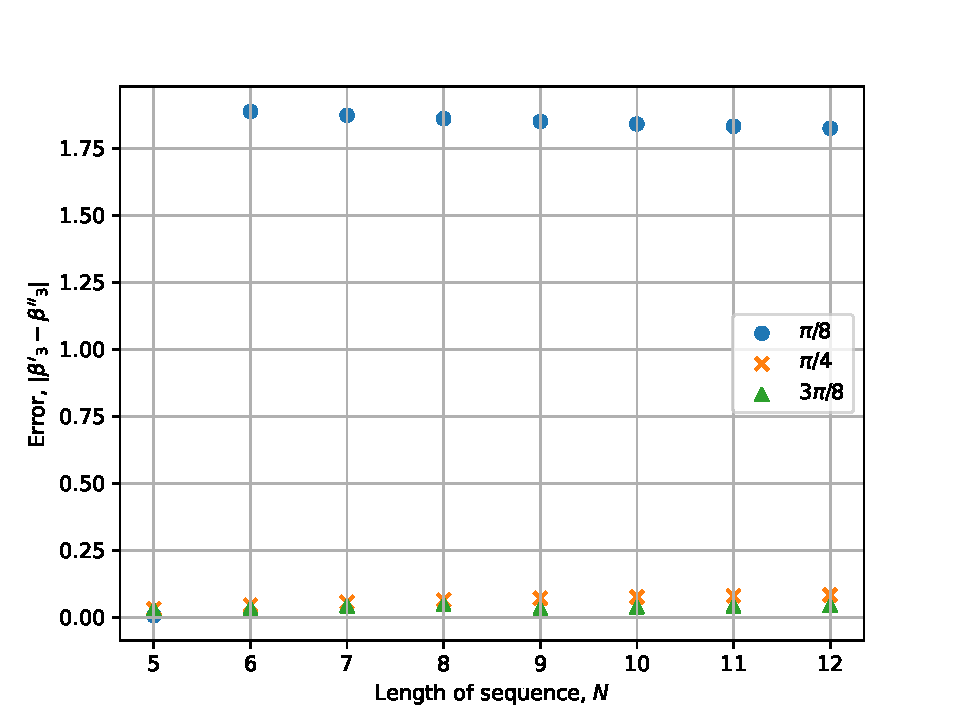
\includegraphics[width=\textwidth]{figs/ch3_QSD/approx_3CP.pdf}
        \caption{Absolute value of the difference between the solution and the heuristic for $\theta \in \{\pi/8, \pi/4, 3\pi/8\}$ as a function of $N$.}
    \end{subfigure}
    \caption{
    The final case is where there are three stages of mutations: 
    (1) from $\ket{0}$ to \\ $\ket{\phi_1} = \cos(\theta) + \sin(\theta)$, then
    (2) from $\ket{\phi_1} = \cos(\theta) + \sin(\theta)$ to $\ket{\phi_2} = \cos(2\theta) + \sin(2\theta)$, and finally
    (3) from $\ket{\phi_2} = \cos(2\theta) + \sin(2\theta)$ to $\ket{\phi_3} = \cos(3\theta) + \sin(3\theta)$, for $\theta \in \{\pi/8, \pi/4, 3\pi/8\}$.
    We contrast the optimal reward function values for varying $\theta$ as a function of the length of the sequence $N$ (on the left), and the absolute difference between the heuristic and the solution (on the right).
    Observe that when $\theta = \pi/8$, the SDP solver is unable to compute the solution and hence~\eqref{eq:ch3_QSD-reduceddual} is assigned of $-1$ for sequences of length larger than $5$.
    More importantly, the heuristic manages to obtain a solution.
    This explains the large error for $\theta = \pi/8$ (on the right) which is more of an indication of the unsolvability than it is an actual error.
    } 
    \label{fig:ch3_QSD-3CP}
\end{figure}

%\section{A2} \label{ase:app_one_sect_2}
% \chapter{Second Appendix} \label{app:appendix_two}
\end{appendices}